\documentclass[12pt, a4paper]{report}

% ─── Encoding & Language ───────────────────────────────────────────────────────
\usepackage[utf8]{inputenc}
\usepackage[T1]{fontenc}
\usepackage[english]{babel}

% ─── Typography ────────────────────────────────────────────────────────────────
\usepackage{lmodern}
\usepackage{microtype}
\usepackage{setspace}
\onehalfspacing

% ─── Page Layout ───────────────────────────────────────────────────────────────
\usepackage[
  top=2.5cm, bottom=2.5cm,
  left=3cm,  right=2.5cm
]{geometry}

% ─── Images ────────────────────────────────────────────────────────────────────
\usepackage{graphicx}
\usepackage{float}
\graphicspath{{images/}}

% ─── Tables ────────────────────────────────────────────────────────────────────
\usepackage{booktabs}
\usepackage{tabularx}
\usepackage{array}
\usepackage{caption}
\captionsetup{font=small, labelfont=bf}

% ─── Code Listings ─────────────────────────────────────────────────────────────
\usepackage{listings}
\usepackage{xcolor}

\definecolor{codegray}{rgb}{0.95,0.95,0.95}
\definecolor{codegreen}{rgb}{0,0.5,0}
\definecolor{codepurple}{rgb}{0.5,0,0.5}
\definecolor{codeblue}{rgb}{0,0,0.6}

\lstdefinestyle{mystyle}{
  backgroundcolor=\color{codegray},
  commentstyle=\color{codegreen},
  keywordstyle=\color{codeblue}\bfseries,
  stringstyle=\color{codepurple},
  basicstyle=\ttfamily\footnotesize,
  breakatwhitespace=false,
  breaklines=true,
  captionpos=b,
  keepspaces=true,
  numbers=left,
  numbersep=5pt,
  showstringspaces=false,
  tabsize=2
}
\lstset{style=mystyle}

% ─── Hyperlinks & PDF Metadata ─────────────────────────────────────────────────
\usepackage[
  colorlinks = true,
  linkcolor  = black,
  urlcolor   = blue,
  citecolor  = black,
  pdftitle   = {MerchStory: AI-Powered Advertisement Generation for Small Retailers},
  pdfauthor  = {Borodi Bogdan-Vasile}
]{hyperref}
\usepackage{bookmark}

% ─── Bibliography ──────────────────────────────────────────────────────────────
\usepackage[backend=biber, style=ieee]{biblatex}
% \addbibresource{references.bib}

% ─── Diagrams ──────────────────────────────────────────────────────────────────
\usepackage{tikz}
\usetikzlibrary{arrows.meta, positioning, shapes.geometric}

% ─── Miscellaneous ─────────────────────────────────────────────────────────────
\usepackage{amsmath, amssymb}
\usepackage{enumitem}

% ═══════════════════════════════════════════════════════════════════════════════
%  TITLE PAGE
% ═══════════════════════════════════════════════════════════════════════════════
\begin{document}

\begin{titlepage}
  \centering
  \vspace*{1.5cm}

  {\large \textbf{Babe\c{s}-Bolyai University, Cluj-Napoca}}\\[0.3cm]
  {\large Faculty of Mathematics and Computer Science}\\[0.3cm]
  {\large Department of Computer Science}

  \vspace{2cm}

  \rule{\linewidth}{0.5pt}\\[0.4cm]
  {\LARGE \bfseries MerchStory: AI-Powered Advertisement\\[0.3cm]
  Generation for Small Retailers}\\[0.4cm]
  \rule{\linewidth}{0.5pt}

  \vspace{1.5cm}

  {\large \textit{Bachelor Thesis --- Laboratory Assignment 2}}

  \vspace{2cm}

  \begin{tabular}{rl}
    \textbf{Author:}      & Borodi Bogdan-Vasile \\[0.2cm]
    \textbf{Supervisor:}  & Horea-Bogdan Mure\c{s}an, PhD \\[0.2cm]
    \textbf{Programme:}   & Bachelor of Computer Science \\[0.2cm]
    \textbf{Year:}        & 2025--2026 \\
  \end{tabular}

  \vfill
\end{titlepage}

% ═══════════════════════════════════════════════════════════════════════════════
%  ABSTRACT
% ═══════════════════════════════════════════════════════════════════════════════
\begin{abstract}
\noindent
The proliferation of e-commerce and social media marketing has created a
significant disparity between large enterprises --- which can afford dedicated
marketing teams and graphic designers --- and small, independent retailers, who
must produce competitive visual content with limited resources and technical
expertise.  \textbf{MerchStory} is a proposed AI-powered mobile application
that aims to close this gap by transforming raw product photographs into
polished, context-aware advertisement assets with minimal user intervention.

\medskip\noindent
The proposed system leverages a provider-agnostic generative image pipeline
orchestrated through Microsoft Semantic Kernel, capable of producing catalog
images, promotional announcements, and scene-composed wallpapers tailored to
each retailer's brand identity.  The back-end is designed as an ASP.NET Core
minimal API (.NET~10) backed by a PostgreSQL~18 relational database, while the
cross-platform mobile client targets iOS, Android, and web from a single
React Native / Expo TypeScript codebase.

\medskip\noindent
This document presents the theoretical foundations of the project, covering
AI-driven image generation techniques, modern cross-platform mobile application
architecture, and secure RESTful API design with token-based authentication.
Subsequent chapters will detail the system design, implementation, and
empirical evaluation of the proposed solution.
\end{abstract}

\clearpage

% ═══════════════════════════════════════════════════════════════════════════════
%  TABLE OF CONTENTS
% ═══════════════════════════════════════════════════════════════════════════════
\tableofcontents
\listoffigures
\listoftables
\clearpage

% ═══════════════════════════════════════════════════════════════════════════════
%  CHAPTER 1 — THEORETICAL BACKGROUND
% ═══════════════════════════════════════════════════════════════════════════════
\chapter{Theoretical Background}
\label{chap:theory}

This chapter presents the theoretical and technical foundations underlying the
MerchStory proposal.  The exposition is organized around three pillars that
correspond directly to the core layers of the system:
(i)~the generative AI techniques considered for synthesizing advertisement
imagery, (ii)~the architectural paradigms adopted for the cross-platform mobile
client, and (iii)~the principles governing secure, scalable RESTful API design
and authentication.  Each section surveys the relevant state of the art and
motivates the design choices proposed for MerchStory.

% ─── 1.1 ───────────────────────────────────────────────────────────────────────
\section{AI-Driven Image Generation}
\label{sec:ai-image-gen}

\subsection{From GANs to Diffusion Models}

The field of AI-generated imagery has undergone a remarkable transformation over
the past decade.  Early successes were dominated by Generative Adversarial
Networks (GANs)~\cite{goodfellow2014generative}, in which a \emph{generator}
and a \emph{discriminator} network are trained in an adversarial minimax game.
While GANs produced visually convincing outputs, training instability,
mode~collapse, and limited compositional reasoning restricted their applicability
to controlled domains.

\medskip\noindent
Denoising Diffusion Probabilistic Models (DDPMs), introduced by
Ho~et~al.~\cite{ho2020denoising}, reframed generation as a learned reverse
Markov chain: a \emph{forward process} gradually corrupts a clean image with
Gaussian noise across $T$ time steps, and a neural network learns to invert
this process step by step.  Latent Diffusion Models
(LDMs)~\cite{rombach2022highresolution} extended this paradigm by performing
diffusion in a compressed \emph{latent space} produced by a
Variational Autoencoder (VAE), drastically reducing computational cost without
sacrificing perceptual quality.  Stable Diffusion, the best-known open-source
LDM, operates on $64{\times}64$ latent representations corresponding to
$512{\times}512$ pixel images, and supports conditioning on text embeddings
produced by a frozen CLIP~\cite{radford2021learning} or T5 encoder.

\medskip\noindent
OpenAI's DALL$\cdot$E~3 and Google's Imagen~3 pushed text-image alignment
further by coupling large language models with cascade diffusion architectures.
DALL$\cdot$E~3 routes user prompts through GPT-4 before passing them to the
image model, ensuring semantic fidelity even for complex compositional
instructions.  Imagen~3 employs cascaded diffusion at multiple resolutions,
producing $1024{\times}1024$ outputs with state-of-the-art photorealism
according to PartiPrompts and COCO benchmarks.

\subsection{Model-Agnostic Generation Architecture}

A central architectural goal of MerchStory is that the image generation layer
be \emph{provider-agnostic}.  The generative AI market is evolving rapidly ---
models such as Google Gemini, OpenAI's DALL$\cdot$E series, Stability AI's
Stable Diffusion XL, and video-generation models such as OpenAI Sora are
continuously advancing, with new entrants regularly achieving state-of-the-art
results on standard benchmarks.  Rather than committing to a single provider,
the proposed architecture routes all generation calls through a common
\texttt{IImageProvider} interface, whose concrete implementation is selected
at configuration time without affecting any business logic --- an application
of the Dependency Inversion Principle of SOLID software engineering.

\medskip\noindent
This abstraction makes the choice of underlying model a deployment decision
rather than an engineering one.  Any provider that accepts a text prompt and
optional reference images and returns pixel data can be wrapped as an
\texttt{IImageProvider} implementation.  Multimodal models are of particular
interest for this domain: unlike text-only conditioned systems, they can attend
simultaneously to a product photograph and a natural-language description of
brand colors, tone, and target audience, enabling stronger visual consistency
with the retailer's existing assets.  Providers such as DALL$\cdot$E~3,
Gemini, or Stable Diffusion XL can thus be treated as interchangeable
back-ends, selectable via dependency-injection configuration with no changes to
route handlers or orchestration logic.

\medskip\noindent
Microsoft Semantic Kernel acts as the orchestration layer above whichever
provider is active, managing prompt template rendering, plugin invocations,
and multi-model routing.  This architecture also supports task-level model
selection: for example, background wallpaper generation (where artistic quality
matters most) could be routed to a different provider than social media
announcement generation (where speed and cost are paramount), all within
Semantic Kernel's planning infrastructure.

\subsection{Prompt Engineering and Brand-Aware Generation}

Effective use of large generative models depends heavily on the quality of
the input prompt.  In a commercial context, a poorly specified prompt may
yield an aesthetically pleasing image that nonetheless fails to communicate
the brand's visual identity or product attributes.  MerchStory addresses this through a structured \texttt{BrandContext} object
that encodes up to 13 optional brand parameters --- including primary and
accent colors, typography preferences, industry domain, and target demographic
--- injected into every generation request as a system-level preamble.
Prompt templates are maintained as structured records rendered at request time
with the user's brand context, externalizing prompt logic from application code
and enabling iteration on generation quality without redeployment.

\subsection{Context Engine, Retrieval-Augmented Generation, and Recommendation}

Beyond static brand context, MerchStory is designed around the principle that
\emph{the best advertisement is also the most timely one}.  The planned
\textbf{Context Engine} enriches every generation request with real-time
signals derived from three sources:

\begin{itemize}[leftmargin=*]
  \item \textbf{Weather} --- current local conditions are queried at generation
    time and mapped to product relevance scores.  For example, a rainy forecast
    triggers increased relevance for comfort-food or accessory promotions, while
    a heatwave elevates cold-beverage and outdoor-gear categories.

  \item \textbf{Local Events and News} --- regional sports results, concerts,
    or community happenings are monitored via public APIs.  When a local team
    wins, the engine may suggest a celebratory-themed ad; when a street market
    is scheduled nearby, it may recommend higher posting frequency.

  \item \textbf{Holidays and Paydays} --- a calendar of standard high-spend
    triggers (national holidays, end-of-month paydays) is maintained and used
    to pre-schedule generation campaigns with appropriate seasonal tone and
    visual style.
\end{itemize}

\medskip\noindent
The longer-term vision incorporates \textbf{Retrieval-Augmented Generation
(RAG)} applied to the user's own photo library.  Product photographs uploaded
by the retailer are encoded into dense vector embeddings using a vision
encoder and stored in the \texttt{pgvector} extension of PostgreSQL~18.
At generation time, a semantic similarity search retrieves the most relevant
previously cleaned product shots or generated backgrounds from the user's
asset history, which are then provided as visual context to the generative
model.  This allows the system to maintain visual consistency across a
retailer's catalogue without requiring manual selection of reference images,
and progressively improves output quality as the asset library grows.

\medskip\noindent
The \textbf{Smart Scheduler} (planned for Phase~2) closes the recommendation
loop: rather than generating ads on demand, Semantic Kernel's planning
infrastructure will analyze historical engagement metrics (clicks, likes,
reach per post) stored in the \texttt{SocialPost} table alongside contextual
signals to propose an optimal posting calendar.  A/B creative testing ---
generating two ad variants and automatically scaling the better-performing
one --- will further refine the recommendation model over time, moving
MerchStory from a generation tool towards a closed-loop retail growth engine.

% ─────────────────────────────────────────────────────────────────────────────
%  TABLE 1.1 — Model Comparison
% ─────────────────────────────────────────────────────────────────────────────
\begin{table}[H]
  \centering
  \caption{Comparison of state-of-the-art text-to-image generation models.}
  \label{tab:model-comparison}
  \begin{tabular}{@{} l >{\raggedright\arraybackslash}p{2.8cm} >{\raggedright\arraybackslash}p{6.2cm} c @{}}
    \toprule
    \textbf{Model}        & \textbf{Provider}   & \textbf{Key Characteristic}        & \textbf{Max Resolution} \\
    \midrule
    DALL$\cdot$E 3        & OpenAI              & GPT-4 prompt rewriting; strong compositional fidelity            & $1024{\times}1024$ \\[3pt]
    Stable Diffusion XL   & Stability AI        & Open-source latent diffusion; large community fine-tune library  & $1024{\times}1024$ \\[3pt]
    Imagen 3              & Google DeepMind     & Cascaded diffusion; top score on PartiPrompts benchmark          & $1024{\times}1024$ \\[3pt]
    Gemini 2.0 Flash      & Google              & Natively multimodal; simultaneous text and image I/O             & $1024{\times}1024$ \\[3pt]
    Midjourney v6         & Midjourney Inc.     & High artistic quality; subscription-based API access             & $2048{\times}2048$ \\
    \bottomrule
  \end{tabular}
\end{table}

\bigskip\noindent
Table~\ref{tab:model-comparison} summarizes the landscape of leading
text-to-image models considered for MerchStory.  Because the system adopts
a provider-agnostic \texttt{IImageProvider} interface, any of the above
models can serve as the active back-end, and the selection can evolve as the
generative AI landscape continues to advance.

% ─────────────────────────────────────────────────────────────────────────────
%  TABLE 1.2 — MerchStory Generation Endpoints
% ─────────────────────────────────────────────────────────────────────────────
\begin{table}[H]
  \centering
  \footnotesize
  \caption{MerchStory image generation endpoints and their supported parameters.}
  \label{tab:generation-endpoints}
  \begin{tabular}{@{} >{\ttfamily\raggedright\arraybackslash}p{4.4cm}
                       >{\raggedright\arraybackslash}p{3.2cm}
                       >{\raggedright\arraybackslash}p{6.6cm} @{}}
    \toprule
    \normalfont\textbf{Endpoint} & \textbf{Output Type} & \textbf{Key Parameters} \\
    \midrule
    /generate-image/\newline catalog
      & Product catalog image
      & Products (name, price, image), layout style, colour theme, aspect ratio, show prices flag \\[6pt]
    /generate-image/\newline wallpaper
      & Background scene
      & Brand context, output format (square / portrait / story) \\[6pt]
    /generate-image/\newline catalog-on-wallpaper
      & Composite product scene
      & Products, wallpaper style, layout, output format \\[6pt]
    /generate-image/\newline announcement
      & Social media post
      & Post type, text content, tone (professional / playful / urgent), output format \\
    \bottomrule
  \end{tabular}
\end{table}

% ─── 1.2 ───────────────────────────────────────────────────────────────────────
\section{Cross-Platform Mobile Application Architecture}
\label{sec:mobile-arch}

\subsection{React Native and the Bridge Architecture}

React Native, released by Meta in 2015, enables developers to write mobile
applications in JavaScript and TypeScript while rendering to genuinely native
UI widgets on both iOS and Android~\cite{eisenman2015learning}.  Unlike
WebView-based hybrid frameworks (such as Apache Cordova), React Native
communicates with native platform APIs through an asynchronous serialized
\emph{bridge}: JavaScript business logic executes on a dedicated JS thread,
while native rendering occurs on the main UI thread, with messages exchanged
in JSON-serialized batches.

\medskip\noindent
The New Architecture (\emph{Fabric} renderer and \emph{JSI} --- JavaScript
Interface) introduced in React Native 0.68 and stabilized in later releases
replaces the asynchronous bridge with synchronous, direct C++ bindings,
enabling mutual object references between JavaScript and native code without
serialization overhead.  React Native Reanimated~v4, used in MerchStory for
animated input fields and transition effects, leverages worklets --- small
JavaScript functions serialized to the UI thread via JSI --- to achieve
60/120\,fps animations that cannot be interrupted by main-thread JavaScript
execution.

\subsection{Expo and File-Based Routing with Expo Router}

Expo is a managed development platform built atop React Native that provides
a unified SDK, over-the-air updates, and a consistent build/deployment
pipeline for iOS, Android, and web from a single codebase.  MerchStory targets
Expo SDK~54 (React Native~0.81, React~19), which ships with the React
Compiler enabled by default, automatically memoizing component trees to reduce
unnecessary re-renders.

\medskip\noindent
\textbf{Expo Router}~v6 introduces a file-system-based routing convention
analogous to Next.js: every file under the \texttt{app/} directory maps to a
route segment, and nested folders create nested navigators automatically.
MerchStory organizes its screens into three route groups:
\texttt{(auth)} for unauthenticated flows (login, register),
\texttt{(setup)} for the onboarding wizard (three-step brand configuration),
and \texttt{(tabs)} for the authenticated main application (home, products,
gallery, analytics, and profile).

\medskip\noindent
This structure produces a clear, auditable mapping between file names and
application screens, lowers the cognitive overhead of adding new screens, and
enables deep-linking out of the box via Universal Links / App Links --- a
requirement for the OAuth callback flow used in the Facebook social
integration.

\subsection{State Management via React Context}

MerchStory eschews heavyweight third-party state management libraries in favour
of React's built-in Context API, which is sufficient for the application's
current scope.  Three contexts are provided:

\begin{enumerate}[leftmargin=*, label=\arabic*.]
  \item \textbf{AuthContext} --- stores the JWT access token, refresh token,
    authenticated user's email, and onboarding completion status.  Tokens are
    persisted to \texttt{expo-secure-store} on native platforms (backed by
    iOS Keychain / Android Keystore) and to \texttt{localStorage} on web.
    On receiving an HTTP~401 response, the context transparently issues a
    refresh-token exchange and retries the original request, exposing this
    behaviour to consumers via a unified \texttt{apiFetch} helper.

  \item \textbf{ShopContext} --- caches the authenticated user's shop profile
    (brand colors, logo, business domain, social handles) fetched from the
    \texttt{/shop/profile} endpoint, avoiding redundant network requests
    across screens.

  \item \textbf{ThemeContext} --- manages dark/light mode preference and
    exposes a toggle function; all color values are resolved from the
    \texttt{constants/theme.ts} token palette rather than being hardcoded
    in component styles.
\end{enumerate}

% ─────────────────────────────────────────────────────────────────────────────
%  FIGURE 1.1 — High-level architecture
% ─────────────────────────────────────────────────────────────────────────────
\begin{figure}[H]
  \centering
  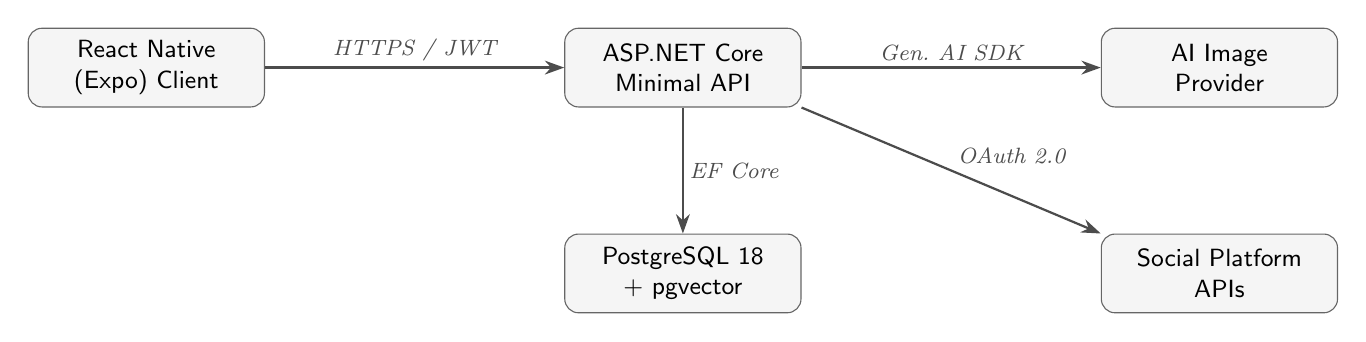
\begin{tikzpicture}[
    node distance = 1.6cm and 3.8cm,
    box/.style = {
      rectangle, rounded corners = 5pt,
      draw = black!60, fill = gray!8,
      minimum width = 3.0cm, minimum height = 1.0cm,
      align = center, font = \small\sffamily
    },
    arr/.style  = {-{Stealth[length=7pt, width=5pt]}, thick, black!70},
    lbl/.style  = {font = \footnotesize\itshape, fill = white, inner sep = 2pt}
  ]
    % ── Nodes ────────────────────────────────────────────────────────────────
    \node[box]                        (client)  {React Native\\(Expo) Client};
    \node[box, right = of client]     (api)     {ASP.NET Core\\Minimal API};
    \node[box, below = of api]        (db)      {PostgreSQL 18\\+ pgvector};
    \node[box, right = of api]        (ai)      {AI Image\\Provider};
    \node[box, below = of ai]         (social)  {Social Platform\\APIs};

    % ── Arrows ───────────────────────────────────────────────────────────────
    \draw[arr] (client.east)  -- node[lbl, above]{HTTPS / JWT}   (api.west);
    \draw[arr] (api.south)    -- node[lbl, right]{EF Core}        (db.north);
    \draw[arr] (api.east)     -- node[lbl, above]{Gen.\ AI SDK}   (ai.west);
    \draw[arr] (api.south east) -- node[lbl, above right]{OAuth 2.0} (social.north west);
  \end{tikzpicture}
  \caption{High-level architecture of the proposed MerchStory system, showing
    the mobile client, the ASP.NET Core back-end, the PostgreSQL database with
    pgvector support, the provider-agnostic AI image generation layer, and the
    social platform integration.}
  \label{fig:architecture}
\end{figure}

% ─── 1.3 ───────────────────────────────────────────────────────────────────────
\section{RESTful API Design and Token-Based Authentication}
\label{sec:api-auth}

\subsection{Minimal API Pattern in ASP.NET Core}

ASP.NET Core Minimal APIs, introduced in .NET~6 and refined in subsequent
releases, offer a lightweight alternative to the controller-based MVC pattern.
Routes are declared directly in \texttt{Program.cs} or in extension methods,
removing the boilerplate of controller classes and attribute routing.  This
approach aligns with microservice and API-first design principles: each
functional domain (authentication, shop management, image generation, gallery,
products, social integration) is encapsulated in a dedicated \emph{route group}
class (e.g., \texttt{AuthRoutes}, \texttt{ImageGenerationRoutes}), keeping
cohesion high and coupling low.

\medskip\noindent
Entity Framework Core~10 is configured with the \texttt{Npgsql} provider to
target PostgreSQL~18.  Migrations are generated via the EF Core design tools
and applied at startup, ensuring schema consistency across environments.  The
data model is organized around five principal entities ---
\texttt{AppUser}, \texttt{ShopProfile}, \texttt{GeneratedImage},
\texttt{Product}, and \texttt{SocialPost} --- related through foreign keys
with cascading delete semantics, reflecting the lifecycle constraint that all
user-owned data is removed upon account deletion.

\subsection{JWT Authentication and the Refresh-Token Pattern}

Stateless authentication via JSON Web Tokens (JWTs)~\cite{jones2015rfc7519}
is the de-facto standard for mobile API security.  A JWT consists of three
Base64URL-encoded components: a \emph{header} specifying the signing
algorithm, a \emph{payload} containing claims (subject, issuer, audience,
expiration), and a \emph{signature} computed with a server-held secret key.
The server never stores issued tokens; validity is asserted by re-verifying
the signature on every request, yielding horizontal scalability without
shared session state.

\medskip\noindent
MerchStory's \texttt{JwtService} issues access tokens with a 15-minute
expiry to limit the exposure window of a compromised token.  To avoid
forcing users to re-authenticate frequently, a \emph{refresh token} ---
a cryptographically random 64-byte sequence stored as a hashed record in
PostgreSQL --- accompanies each login response.  Mobile clients receive a
refresh token valid for 30~days; web clients receive one valid for 1~day,
reflecting the elevated security sensitivity of browser storage.  When
an access token expires, the client presents the refresh token at the
\texttt{/auth/refresh} endpoint to receive a new access/refresh token pair;
the old refresh token is immediately revoked, implementing
\emph{token rotation} to prevent replay attacks.

\medskip\noindent
A background \texttt{RefreshTokenCleanupService} periodically scans the
\texttt{RefreshTokens} table and purges expired or revoked entries,
bounding the growth of the token table over time without manual
administrative intervention.

\subsection{API Security and Data Transfer Objects}

All authenticated endpoints require a valid JWT in the
\texttt{Authorization: Bearer <token>} header and are protected by
ASP.NET Core's built-in authorization middleware.  Request bodies are
validated using data annotations and minimal API's built-in binding,
ensuring that malformed or incomplete payloads are rejected at the
framework boundary with an HTTP~400 response before reaching business
logic.

\medskip\noindent
Data Transfer Objects (DTOs) decouple the public API contract from the
internal domain model: \texttt{AuthDtos.cs} defines typed request and
response records for registration, login, and token refresh, preventing
accidental exposure of sensitive database fields (e.g., hashed passwords,
internal identifiers) in API responses.  On the frontend, a centralized
API client (\texttt{utils/api.ts}) mirrors these contracts as TypeScript
interfaces, providing end-to-end type safety from the React Native
component down to the HTTP wire format.

% ─────────────────────────────────────────────────────────────────────────────
%  TABLE 1.3 — Authentication endpoint summary
% ─────────────────────────────────────────────────────────────────────────────
\begin{table}[H]
  \centering
  \caption{MerchStory authentication endpoints, HTTP methods, and token
    lifetime configuration.}
  \label{tab:auth-endpoints}
  \begin{tabularx}{\textwidth}{@{} l l X c @{}}
    \toprule
    \textbf{Endpoint}      & \textbf{Method} & \textbf{Description}
      & \textbf{Token Lifetime} \\
    \midrule
    \texttt{/auth/register} & POST  & Create new account; returns JWT + refresh token
      & Access: 15 min \\
    \texttt{/auth/login}    & POST  & Authenticate with email/password
      & Access: 15 min \\
    \texttt{/auth/refresh}  & POST  & Exchange refresh token for new token pair (rotation)
      & Mobile RT: 30 d \\
    \bottomrule
  \end{tabularx}
\end{table}

% ═══════════════════════════════════════════════════════════════════════════════
%  CHAPTER 2 — SYSTEM DESIGN (placeholder)
% ═══════════════════════════════════════════════════════════════════════════════
\chapter{System Design}
\label{chap:design}

\textit{(This chapter will be completed in a subsequent laboratory assignment.)}

\section{Requirements Analysis}
\label{sec:requirements}

\section{Database and Storage Architecture}
\label{sec:db-storage}

\section{API Design}
\label{sec:api-design}

% ═══════════════════════════════════════════════════════════════════════════════
%  CHAPTER 3 — IMPLEMENTATION (placeholder)
% ═══════════════════════════════════════════════════════════════════════════════
\chapter{Implementation}
\label{chap:implementation}

\textit{(This chapter will be completed in a subsequent laboratory assignment.)}

\section{Backend Service}
\label{sec:backend}

\section{Frontend Application}
\label{sec:frontend}

\section{AI Integration}
\label{sec:ai-integration}

% ═══════════════════════════════════════════════════════════════════════════════
%  CHAPTER 4 — EVALUATION (placeholder)
% ═══════════════════════════════════════════════════════════════════════════════
\chapter{Evaluation and Testing}
\label{chap:eval}

\textit{(This chapter will be completed in a subsequent laboratory assignment.)}

\section{Test Strategy}

\section{Results and Discussion}

% ═══════════════════════════════════════════════════════════════════════════════
%  CHAPTER 5 — CONCLUSION (placeholder)
% ═══════════════════════════════════════════════════════════════════════════════
\chapter{Conclusion}
\label{chap:conclusion}

\textit{(This chapter will be completed in a subsequent laboratory assignment.)}

% ═══════════════════════════════════════════════════════════════════════════════
%  BIBLIOGRAPHY (placeholder entries — replace with real .bib file)
% ═══════════════════════════════════════════════════════════════════════════════
% \printbibliography[heading=bibintoc]

\end{document}
